
\begin{frame}[t]{\inhibitglue 誰?}
  \sffamily

  \begin{itemize}
    \item IT系の技術書を世に出す仕事
  \end{itemize}

\end{frame}

\begin{frame}[t]{\inhibitglue 過去の主な仕事}
  \sffamily

  \begin{itemize}
    \item IT系の技術書を世に出す仕事(過去)
  \end{itemize}

  \begin{tabular}{c c c c c}
    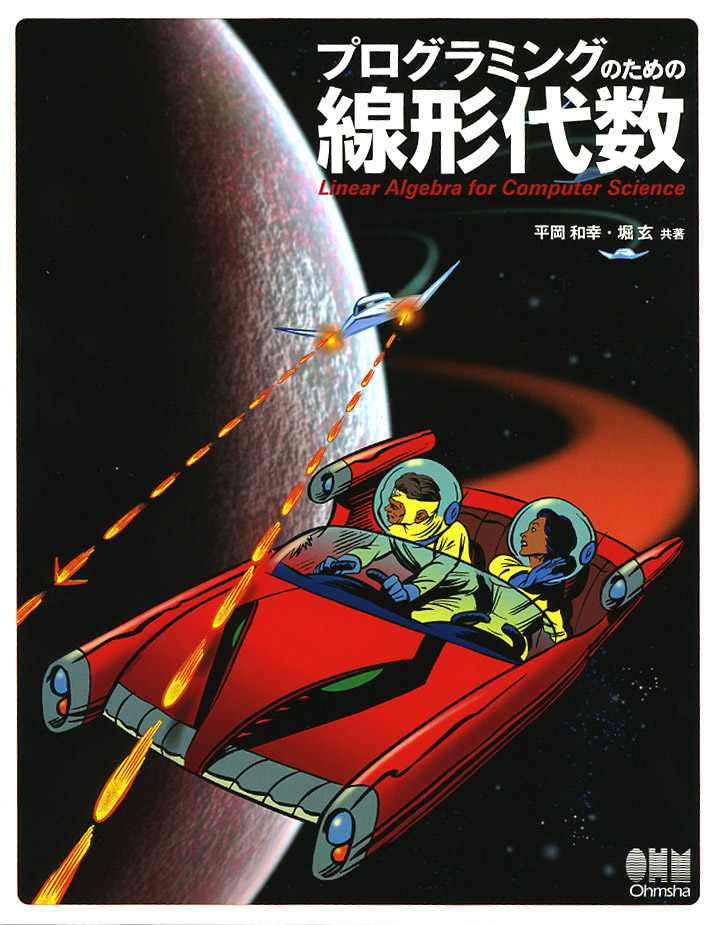
\includegraphics[width=.17\textwidth]{images/4-274-06578-2.jpg}     &
%    
\includegraphics[width=.17\textwidth]{images/978-4-274-06714-3.jpg} &
    
\includegraphics[width=.17\textwidth]{images/978-4-274-06876-8.jpg} &
    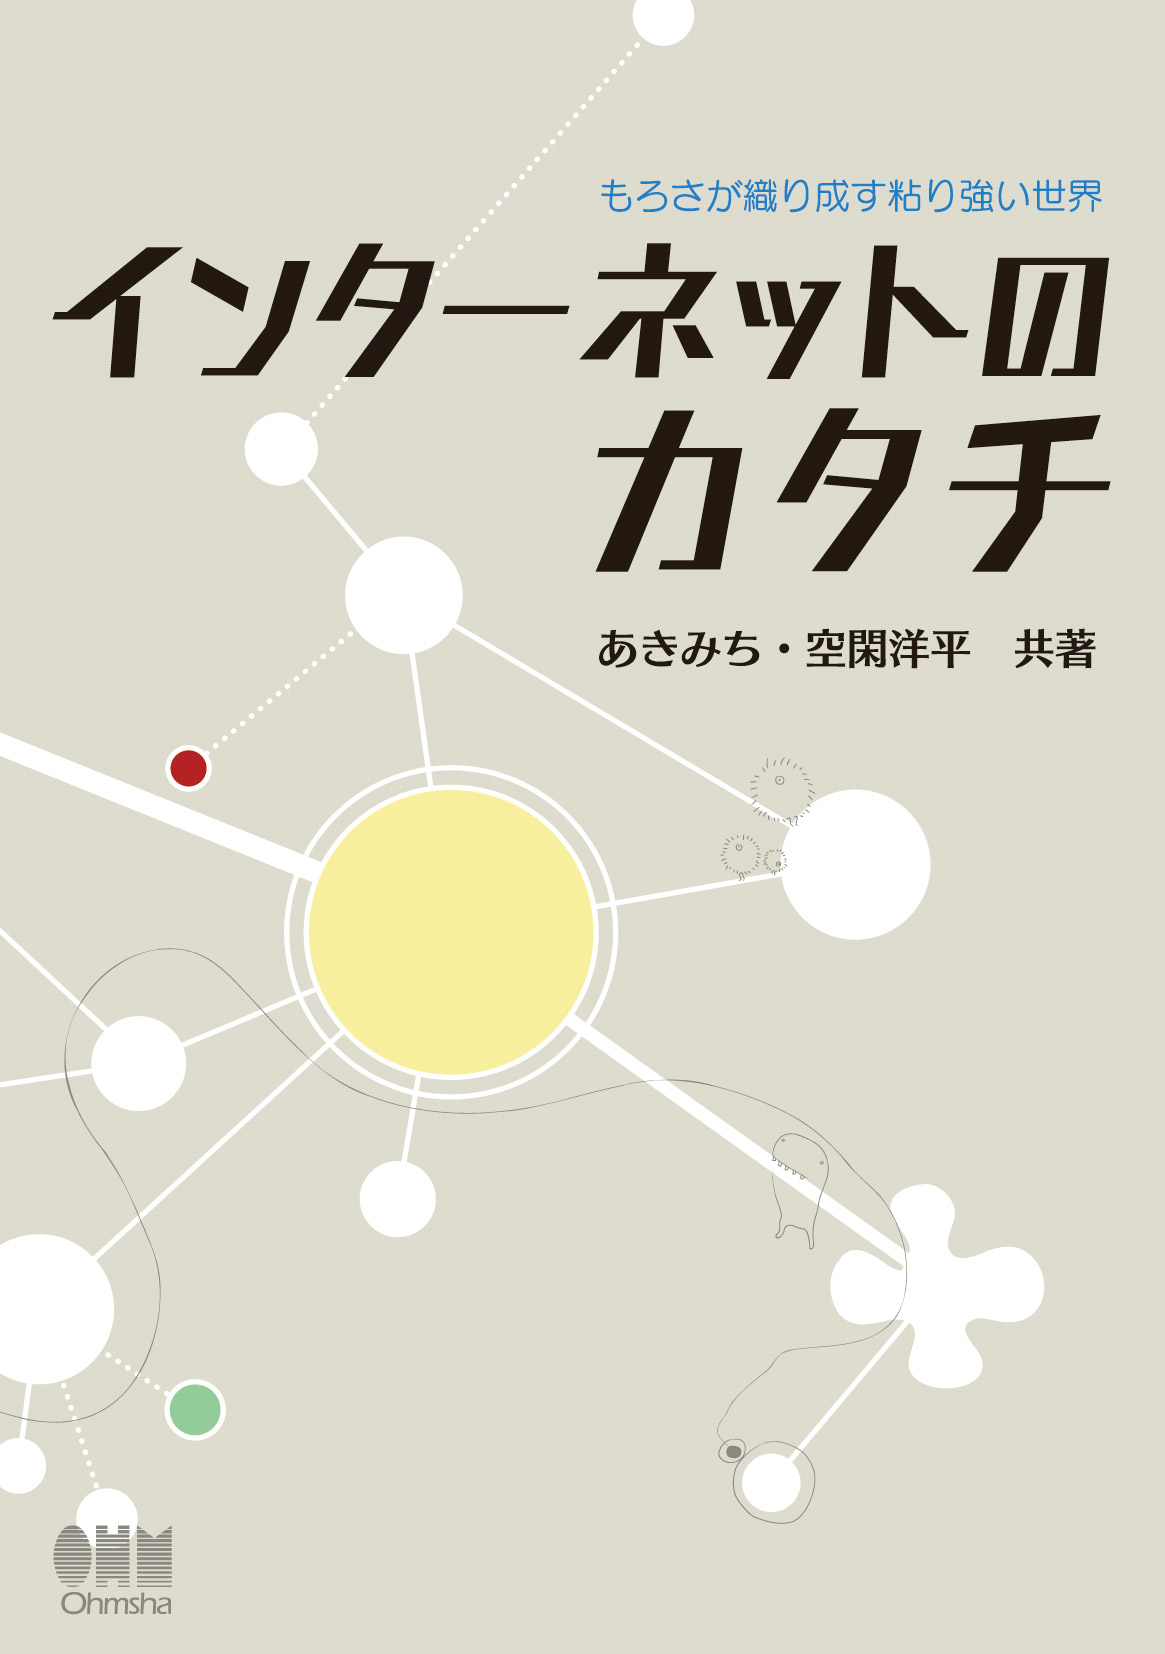
\includegraphics[width=.15\textwidth]{images/978-4-274-06824-9.jpg} &
    
\includegraphics[width=.15\textwidth]{images/978-4-274-06767-9.jpg} &
    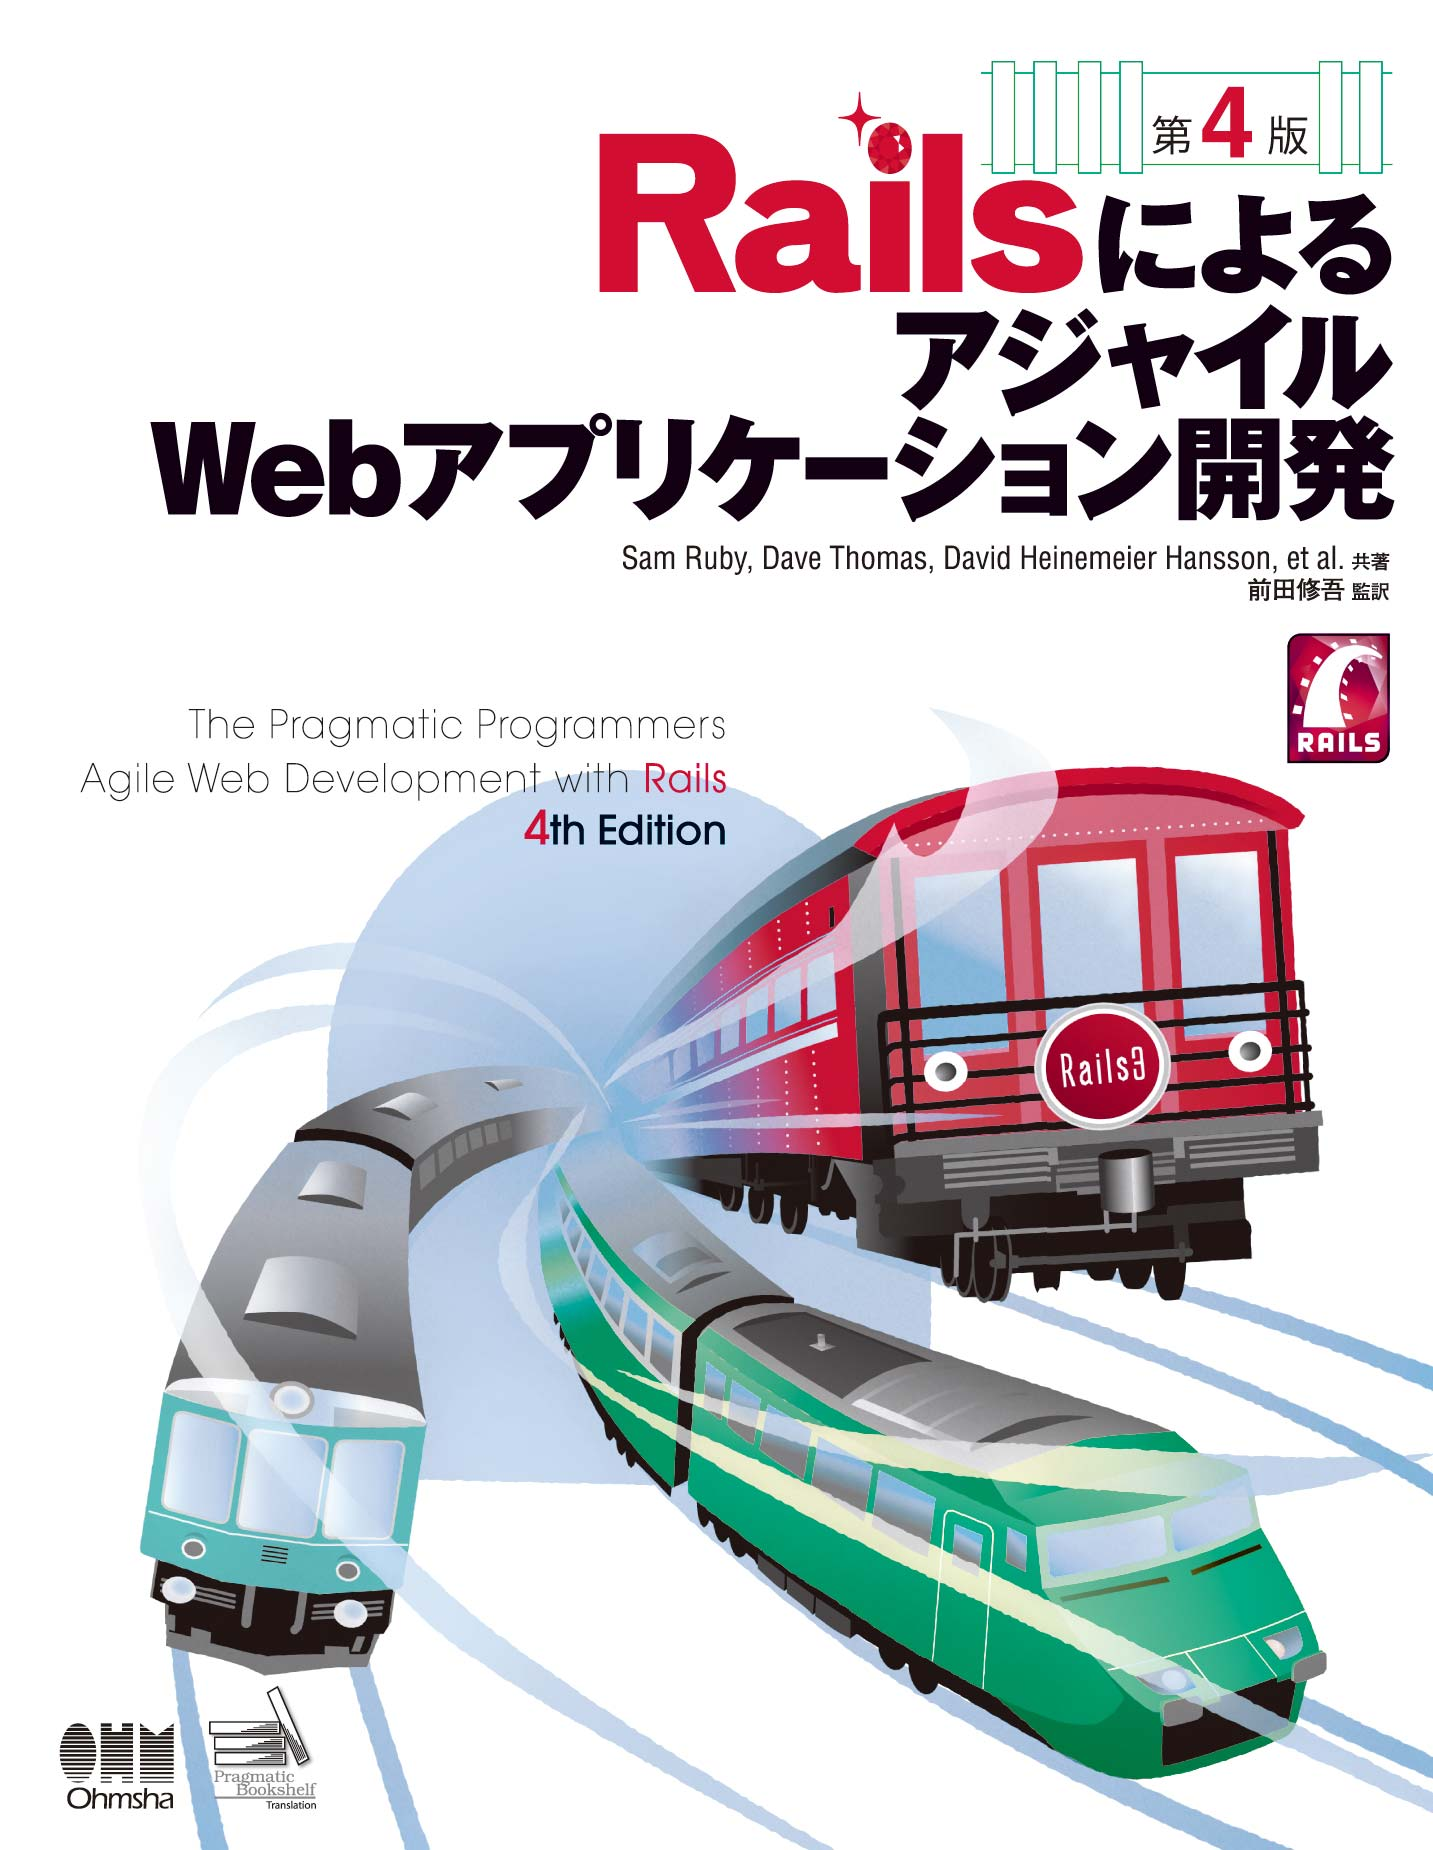
\includegraphics[width=.17\textwidth]{images/978-4-274-06866-9.jpg} \\
    
\includegraphics[width=.17\textwidth]{images/978-4-274-06944-4.jpg} &
    
\includegraphics[width=.17\textwidth]{images/978-4-274-06911-6.jpg} &
    
\includegraphics[width=.15\textwidth]{images/978-4-274-06885-0.jpg} &
    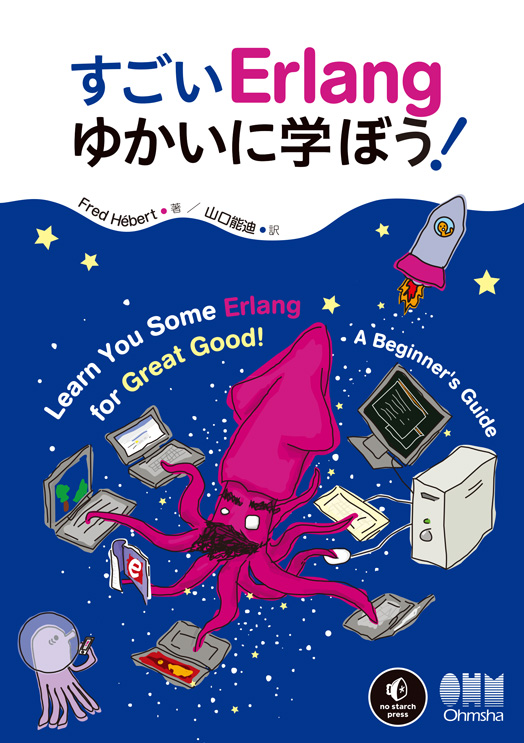
\includegraphics[width=.15\textwidth]{images/978-4-274-06912-3.jpg} &
    
\includegraphics[width=.15\textwidth]{images/978-4-274-21762-3.jpg} 
  \end{tabular}
\end{frame}

\begin{frame}[t]{\inhibitglue 職務経歴書}
  \sffamily

  \begin{itemize}
    \item IT系の技術書を世に出す仕事
    \item 職務経歴書:{\footnotesize \url{http://note.golden-lucky.net/2015/09/blog-post.html}}
  \end{itemize}

\begin{tikzpicture}
  \node at (0,0){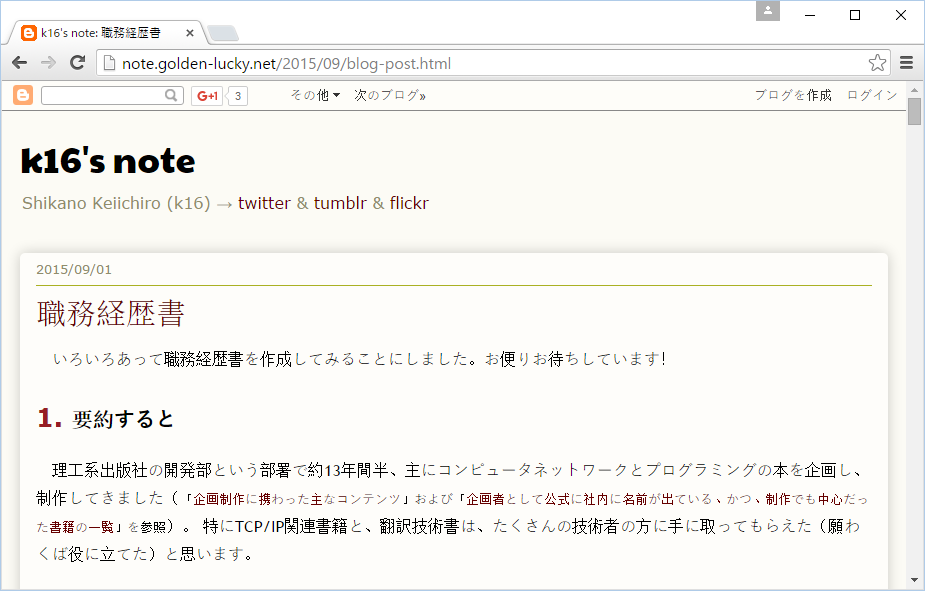
\includegraphics[width=.7\textwidth]{images/kereki1.png}};
\end{tikzpicture}

\end{frame}

\begin{frame}[t]{\inhibitglue 制作システムの開発}
  \sffamily

  \begin{itemize}
    \item IT系の技術書を世に出す仕事
    \item 職務経歴書:{\footnotesize \url{http://note.golden-lucky.net/2015/09/blog-post.html}}
  \end{itemize}

\begin{tikzpicture}
  \node at (0,0){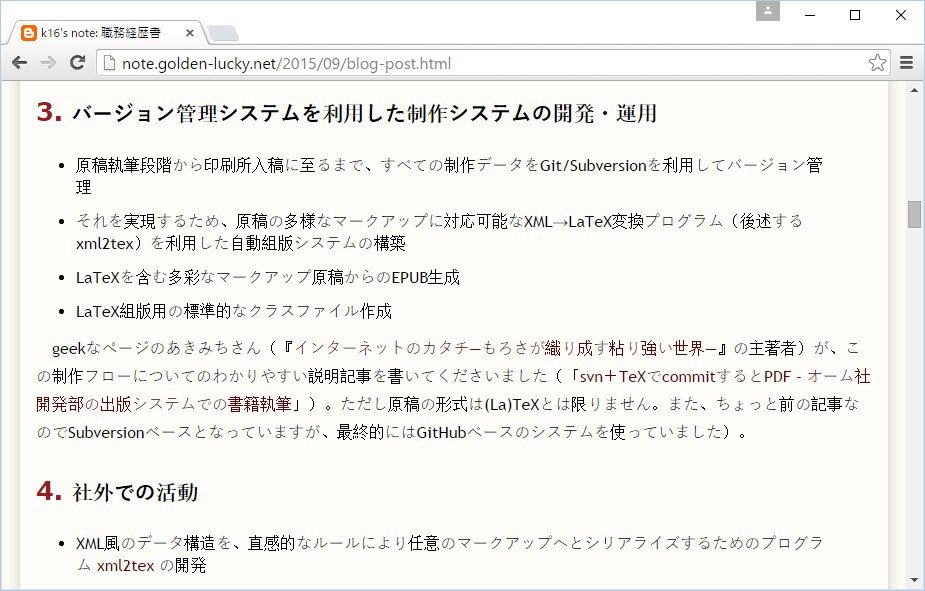
\includegraphics[width=.7\textwidth]{images/kereki2.png}};
  \pause;
  \node[notice={(-1,0.5)}, text width=4.5cm] at (0,-0.5) {自動組版システム?};
  \pause;
  \node[notice={(1,-1)}, text width=1.7cm] at (2,-2) {WTF?};
\end{tikzpicture}

\end{frame}

\begin{frame}[t]{\inhibitglue 版管理+自動組版システム}
  \sffamily

  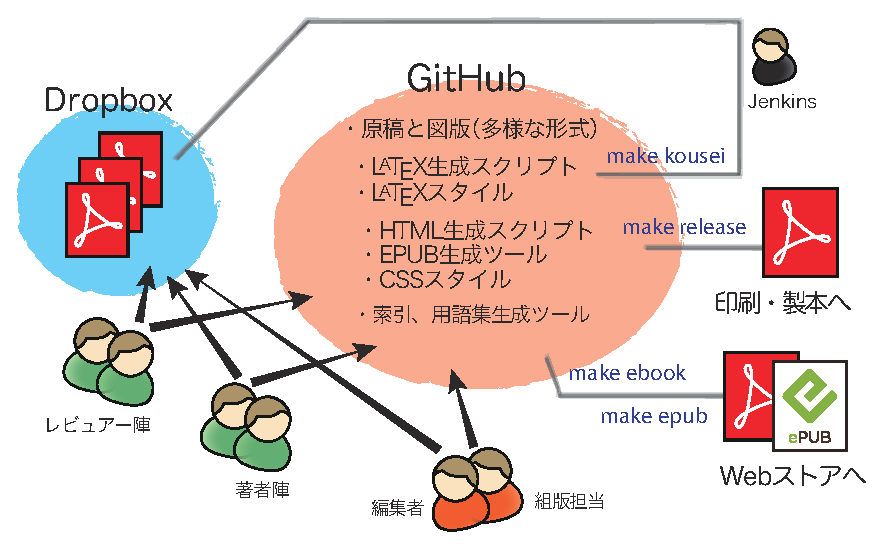
\includegraphics[width=1\textwidth]{images/vcs-centric.pdf}

\end{frame}

\begin{frame}[t]{\inhibitglue 版管理+自動組版イベント}
  \sffamily

\begin{tikzpicture}
  \node at (0,0){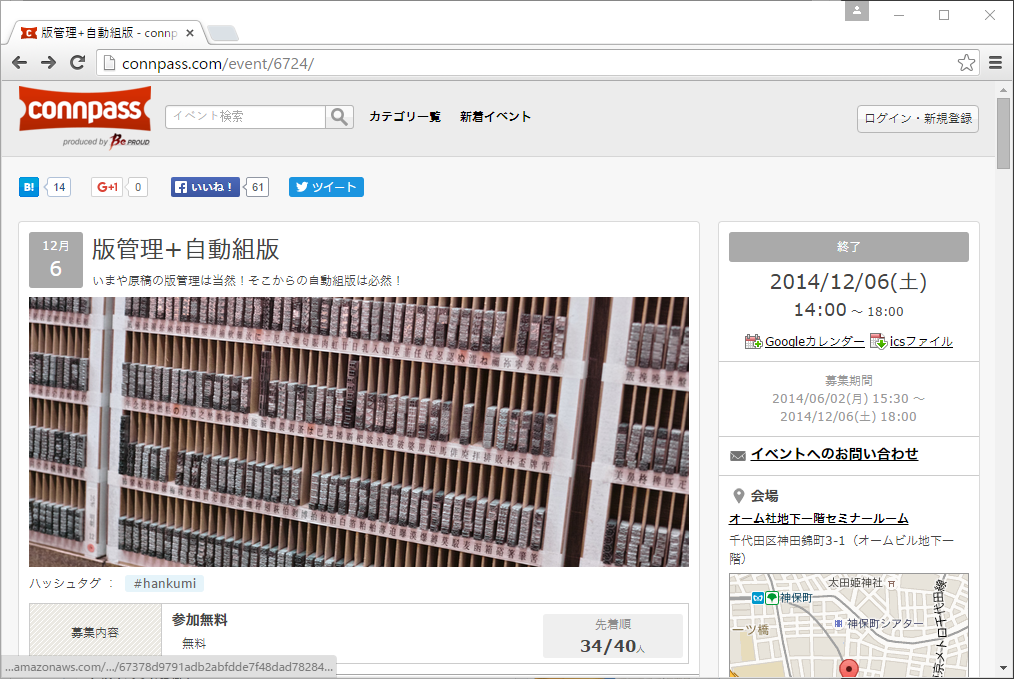
\includegraphics[width=.9\textwidth]{images/hankumi.png}};
  \pause;
  \node[notice={(-2.5,1)}, text width=4cm] at (-2,0) {いつかは第2回!};
\end{tikzpicture}

\end{frame}


